\title{Observations of seismic attenuation changes during CO$_2$ injection in the Frio site, Texas USA}

\author{Tieyuan Zhu$^1$, Jonanthan Ajo-Franklin$^2$, Thomas Daley$^2$ and Sergey Fomel$^1$, \\
$^1$The University of Texas at Austin; $^2$Lawrence Berkeley National Lab}
\maketitle

\righthead{Attenuation}

\begin{abstract}
We investigate spatial-temporal changes in the seismic attenuation of the first arrivals during CO$_2$ injection in the Frio CO$_2$ sequestration brine pilot site. The attenuation changes over the injection period are estimated by the amount of the centroid frequency shift computed by the local frequency tool. Observations are: at receivers above the packer seismic attenuation does not change in a physical trend; at receivers below the packer attenuation sharply increases as the amount of CO$_2$ plume increase and peaks at specific points with distributed receivers, which are consistent with observations from time delays of first arrivals. Then, attenuation decreases over the injection time with increased amount of CO$_2$ plume. The attenuation change shows a unique increase-decrease pattern. Along with the attenuation-saturation White patchy model, the relationship between increase-decrease pattern of attenuation change and CO$_2$ saturation can be (at least) qualitatively explained. Our analysis suggests that seismic attenuation during CO$_2$ injection not only is able to reveal the movement/saturation of CO$_2$ plume but also is sensitive to a possible larger saturation that velocity does not.
\end{abstract}

\section{Introduction: Frio-II field site and monitoring data}
We studied a crosswell seismic monitoring data from the Frio-II brine pilot site. The Frio-II project was a small-scale injection of supercritical CO$_2$ into a high quality reservoir at the same site as the larger Frio-I test in southeast Texas, USA (Hovorka et al., 2006). About 380 tons of CO$_2$ were injected into the Blue sand of the Frio formation. The fluvial Blue sand is at a depth of 1657 m, is 17 m thick, and has a dip of 18 degree, with about 30% porosity and permeability of 1 to over 4 Darcies. 

The experiment site had two wells, the down-dip injector and a dedicated, up-dip, observation well, 30 m apart. In the observation well, we have 13 sensors with variable spacing (5 above the packer and 8 below). The sensor locations included depths above and below the packer, which was deployed at the top of the reservoir sand and above the perforations, as shown in Figure 1a. Crosswell CASSM uses fixed location source and sensors in boreholes to continuously monitor seismic waveforms as they are modified by injecting CO$_2$ (Daley et al., 2007). CO$_2$ injection began at approximately 7:30 pm, Central Daylight Time, on Sep 25, 2006. About 60 hours of continuous monitoring of crosswell seismic response provided information on the spatial and temporal variation of the CO$_2$ plume as it migrated across different raypaths between source-receiver pairs (Figure 1). 

 \begin{figure}[!htb]
   \centering
   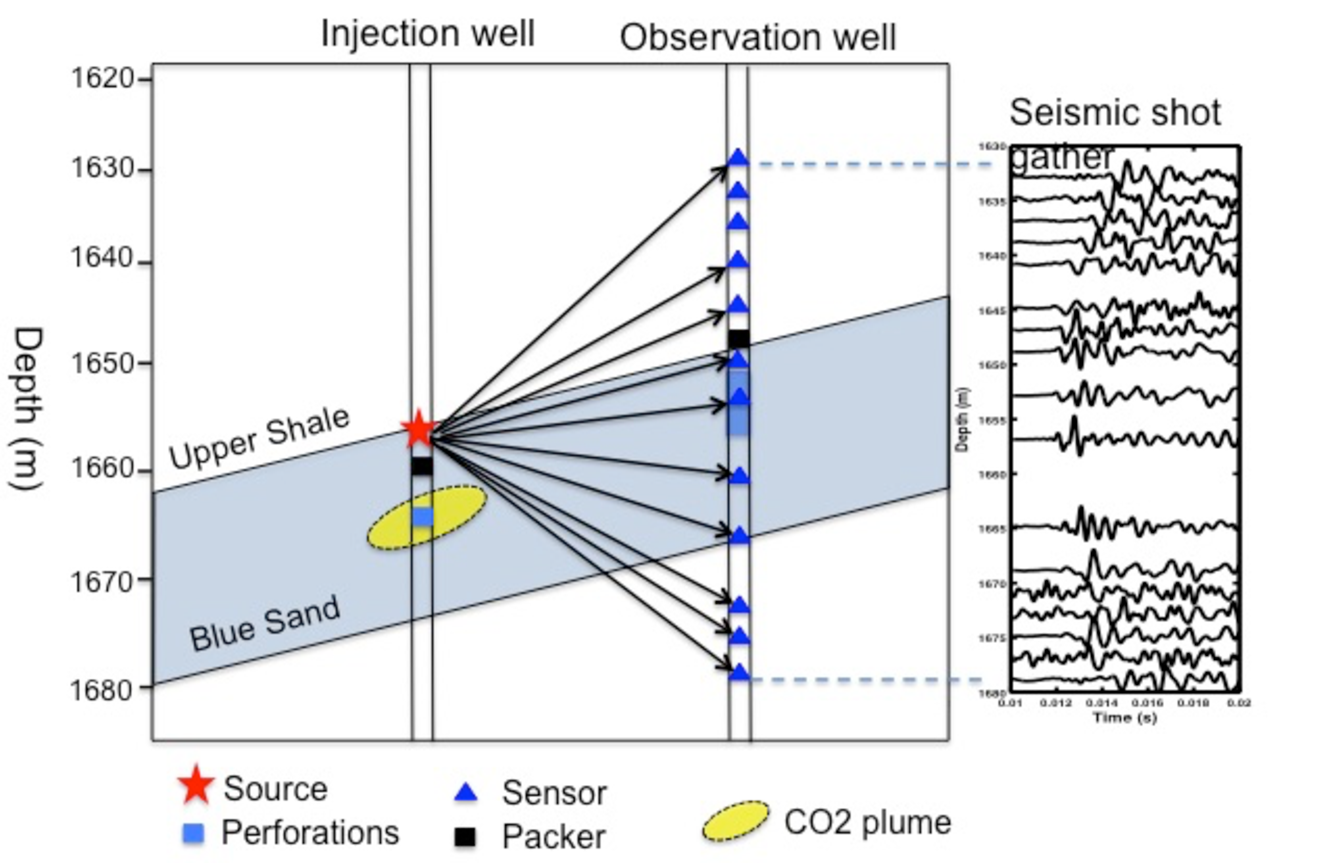
\includegraphics[width=0.4\textwidth]{Fig/fig1}
   \caption{Top: forward propagation in attenuating media; Bottom: backpropagation wavefield in attenuating media with attenuation compensation. The red star denotes an explosive source and the black triangulars denote receivers. The label \textbf{H} and \textbf{L} represent high frequencies and low frequencies signals. To correctly account for attenuation effects (including absorption and phase dispersion), the absorption term must be reversed so as to amplify the signal as time progresses. In contrast, the dispersion term (dependence of the sound speed on frequency) must remain unchanged.}
 \end{figure}
 
To enhance the signal-to-noise ratio (SNR) of the individual source pulse data, we further stacked the raw seismograms in sets of 3600 pulses. This stack processing leads to a series of full seismic data gathers on approximately 15 min intervals during the injection. The partial section of the stacked seismic data at four different receivers is shown in Figure 1b. In the previous studies (Daley et al., 2007; Daley et al., 2011), we extracted delay time (change in crosswell travel time) as a function of the calendar time from our seismic data. As seen in Figure 1b, the different raypaths show different traveltime characteristics of the first arrival in both the magnitude of traveltime and the time of change. Notable is the large traveltime change observed on the 1650 m sensor (at the top of the reservoir) and the near zero delay-time change seen on the 1630 m sensor (in the shale caprock, because the shale unit is relatively impermeable and CO$_2$ is not expected to migrate up). This continuous traveltime data is ideal for constraining the modeled spatiotemporal evolution of the CO$_2$ plume and thus improving a flow model’s predictive capabilities.

\section{Theory}
In this study, we analyzed seismic attenuation changes over 60 h period during CO$_2$ injection. Seismic attenuation is measured by using the centroid frequency (CF) shift (Quan and Harris, 1997). We focused on the first arrivals of crosswell seismic data. We used a local frequency technique to compute the CF map of the first arrival energy; we were following the approach described by Liu et al. (2011). The centroid frequency at a given time is defined as
\begin{equation}
\label{eq:eq1}                      
\hspace{0pt} f_{cf}(t)=\frac{\int fF(t,f)df}{\int F(t,f)df},\hspace{\linewidth minus\linewidth}
\end{equation}
where $F(t,f)$ is the time-frequency map defined by time-varying Fourier coefficients constrained by shaping regularization (Fomel, 2007; Liu et al., 2011), $t$ is the trace time, and $f$ is the frequency. For each seismic trace, we will obtain a CF curve $f_{cf}(t)$  with respect to $t$. Then the maximum CF value of each trace $f_{mcf}=max[f_{cf}(t)]$ is picked. We define the temporal variation of the CF with the calendar time $T$: $f_{mcf}(T)$.
Following the theory of the centroid frequency shift (Quan and Harris, 1997), we define attenuation coefficient $\alpha_{0}$ along the raypath (distance is $d$ )
\begin{equation}
\label{eq:eq2}                      
\hspace{0pt} \alpha _0d=\frac{f_{mcf}^S-f_{mcf}^R}{\sigma _{S}^{2}},\hspace{\linewidth minus\linewidth}
\end{equation}

where $f_{mcf}^S$ and $f_{mcf}^R$  are the CF of the signals at source and receivers. The variance $\sigma_{S}^{2}$ of source signal  is defined (Quan and Harris, 1997) as 
\begin{equation}
\label{eq:eq3}                      
\hspace{0pt} \sigma_{S}^{2}=\frac{\int \left ( f-f_{cf}^S \right )^2 F(t,f)df}{\int F(t,f)df},\hspace{\linewidth minus\linewidth}
\end{equation}

In practice, the source signature will not be available but it is same for all receivers so we chose a reference value for all receivers. For example, we chose the mean value of receiver variance   at the top receiver (least disturbs) in the below calculations. It would not affect the attenuation changes among all receivers, though it might result in errors to the absolute attenuation changes within a single receiver. At a specific receiver, we assume that the ray path is a straight ray over the injection time since the velocity change often is several percent ( $d$ keeps unchanged). The centroid frequency of the source is identical due to high repeatability of the source, i.e., $f_{mcf}^S$ keeps constant in temporal. At the same receiver, therefore, temporal attenuation changes  caused by CO$_2$ injection can be defined as
\begin{equation}
\label{eq:eq4}                      
\hspace{0pt} \Delta \alpha =\frac{ f_{mcf}^R (T)- f_{mcf}^R (0)}{d\sigma_{S}^{2}},\hspace{\linewidth minus\linewidth}
\end{equation}

where $T$ represents the injection (calendar) time, $\alpha^{0}$ is the attenuation before CO$_2$ injection, $\Delta \alpha =\alpha(T)-\alpha^{0}$ is the relative attenuation change to $\alpha^{0}$. 

An example of the unprocessed seismic waveform is shown in Figure 2a, which depicts a shot gather at the depth of 1680 m over the period 60 hours after injection. Significant reductions in apparent velocity are visible after injection while a slight weak amplitude can be seen after 40 hours injection. Figure 2b show the first arrivals selected by a 3-ms length Gaussian window. With prior tests, the 80-points smoothing window required by regularization (Fomel, 2007) gives the satisfied resolution in the time and frequency when computing the time-frequency distribution. Figure 2c shows the centroid frequency map for the first arrivals in Figure 2b. The main frequencies are distributed along the first arrivals. Outside the area of the first arrivals frequencies are not zero but smaller than 900 Hz. As results in Figure 2c, high frequencies are at the first six hours of injection and then have a significant reduction in the sections between six and fifteen hours, and high frequencies seem to gradually recover with the sharp transition at around 40 hours. We can clearly see that the trough of the centroid frequency appear at around 10 hours corresponds to the largest time delay (Daley et al., 2007). Figure 2d

 \begin{figure}[!htb]
   \centering
   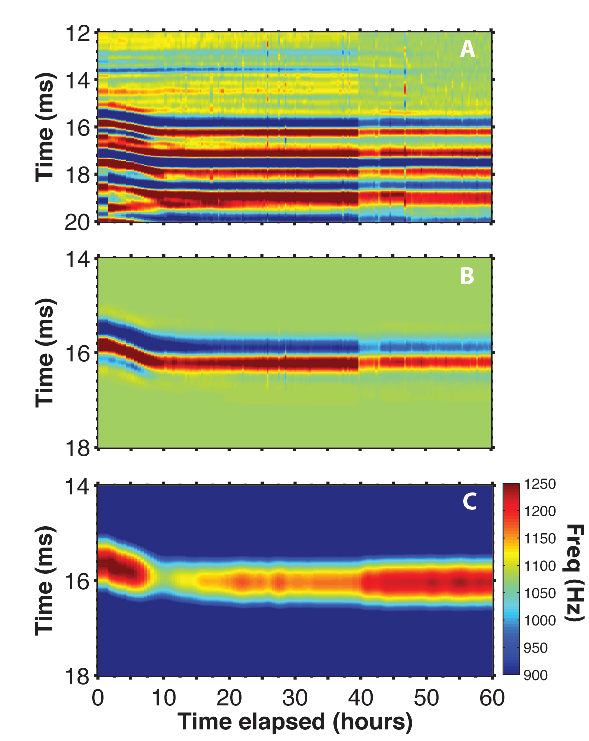
\includegraphics[width=0.4\textwidth]{Fig/fig2}
   \caption{Top: forward propagation in attenuating media; Bottom: backpropagation wavefield in attenuating media with attenuation compensation. The red star denotes an explosive source and the black triangulars denote receivers. The label \textbf{H} and \textbf{L} represent high frequencies and low frequencies signals. To correctly account for attenuation effects (including absorption and phase dispersion), the absorption term must be reversed so as to amplify the signal as time progresses. In contrast, the dispersion term (dependence of the sound speed on frequency) must remain unchanged.}
 \end{figure}
 
\section{Spatial-temporal centroid frequency changes}
Figure 3 shows the maximum centroid frequency values of the first arrivals with the calendar time at four typical sensors, at the depths of 1630 m, 1647 m, 1650 m, 1670 m, and 1680 m from top to bottom. Data from five sensors are placed alongside the schematic raypaths to show the spatial-temporal relationship of the measured CF and attenuation changes in Figure 1. The deeper sensors (1680 and 1670 m) show a sharp drop in the centroid frequency beginning only 3–4 hours after injection with increase after about 10 hours. The peak frequency shifts are about 200 Hz at the depth 1680 m and about 100 Hz at the depth 1670. The 1658-m sensor shows amore gradual decrease in centroid frequency beginning at about 15 hours after injection and arriving at about 80-Hz shifts at about 22 hours. The CF at the 1650-m sensor, which has a raypath along the top of the reservoir, begins to shift up after injection and decreases after about 40 hours. The CF shift is up to 360 Hz. At the 1648 sensor (right below the packer), the trend of frequency shift is quite similar to the 1650-m sensor. The CF shift is about 150-Hz. The location of the lowest CF is shifted towards the later calendar time in four receivers from 1680 m to 1648 m. The observed centroid frequency shift of 50 to 200 Hz represent $2\%$ to $20\%$ changes in centroid frequency. Above the packer 1630 m and others not shown, there is no significant, systematic change in centroid frequency. No clear trend in frequency shifts above the packer demonstrates that the below-packer changes are in the subsurface and that the near-source volume has not been affected by the CO2 injection. Therefore, the observed frequency shifts are real and can be interpreted in terms of CO2 plume migration and/or saturation changes. The grey area represents the standard deviation (~26 Hz) of measured CF variations of the first arrivals collected at depth of 1630 m in the preinjection.

\begin{figure}[!htb]
   \centering
   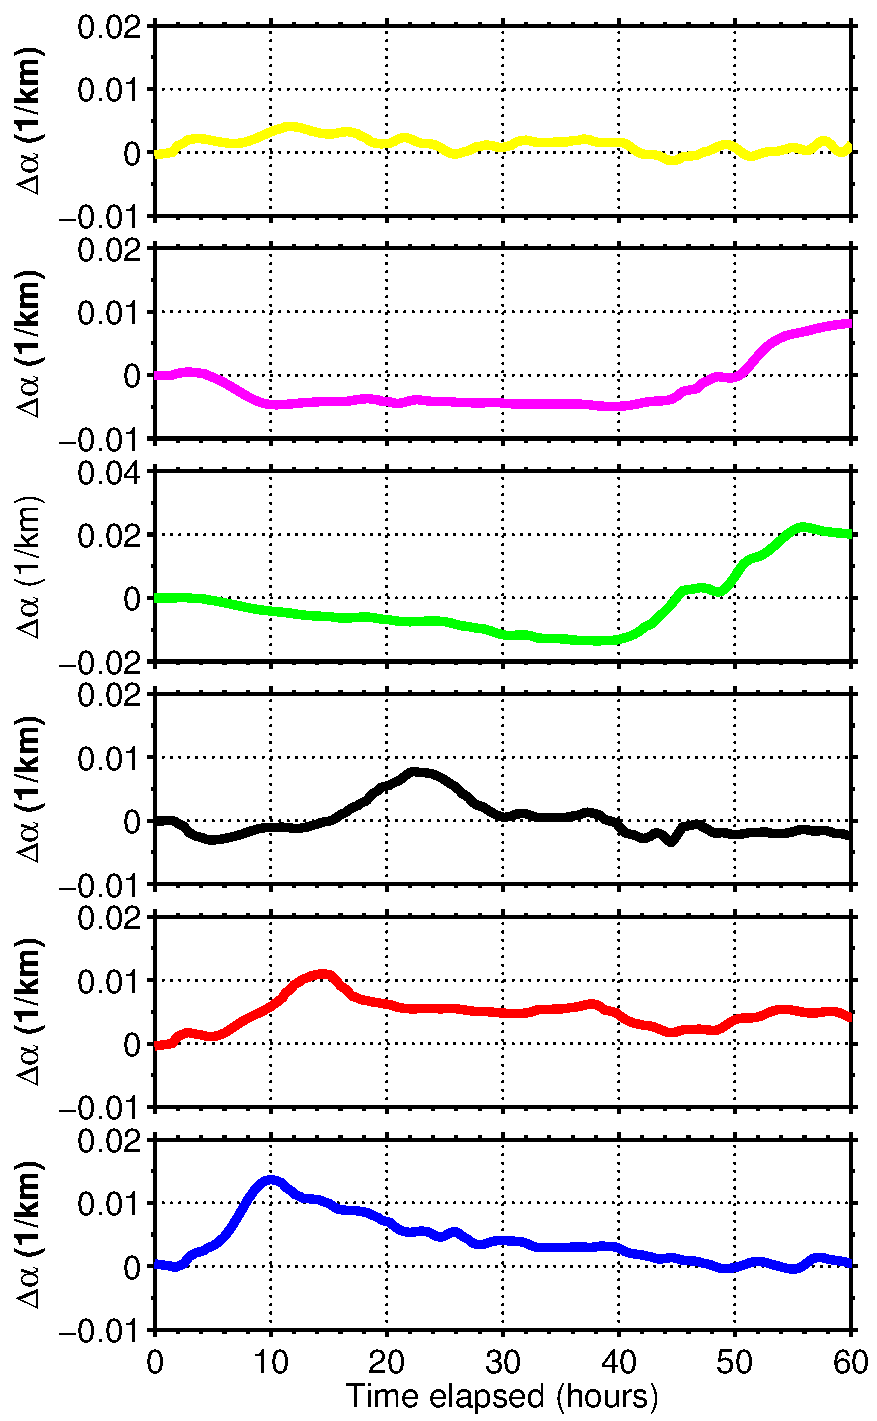
\includegraphics[width=0.4\textwidth]{Fig/fig4}
   \caption{Top: forward propagation in attenuating media; Bottom: backpropagation wavefield in attenuating media with attenuation compensation. The red star denotes an explosive source and the black triangulars denote receivers. The label \textbf{H} and \textbf{L} represent high frequencies and low frequencies signals. To correctly account for attenuation effects (including absorption and phase dispersion), the absorption term must be reversed so as to amplify the signal as time progresses. In contrast, the dispersion term (dependence of the sound speed on frequency) must remain unchanged.}
 \end{figure}
 
\section{Spatial-temporal attenuation changes}
The attenuation changes are computed by using equation 4, as shown in Figure 4. It is assumed that straight raypath is constant during CO$_2$ injection. Below the packer (1647 m), the attenuation changes display three main common features: (1) Small attenuation or negative at the beginning of injection (before the CO$_2$ plume move cross the corresponding raypath), (2) a significant increase in the middle section, and (3) attenuation seems to gradually decrease. Small attenuation (feature 1) is clearly observed at the sensors in the depths of between 1680 m and 1658 m. As seen at sensors in the depths of 1650 m and 1648 m, attenuation after injection seems likely to decrease compared to the preinjection, particularly at the 1650 m sensor. Differential pressure at the top reservoir decrease when Overburden should be static so effective stress should decrease as pore pressure increases during injection (hence lower Q). When CO$_2$ plume move forward and cross the raypath, attenuation starts to increase and is up to a peak positive value (feature 2) that is likely related to the amount of CO$_2$ (saturation). The amount of the attenuation change between sensors is likely to reveal the migration speed of CO$_2$ plume and thus heterogeneities in the reservoir. In feature 3, attenuation then significantly decreases as CO$_2$ plume continues to migrate. It is likely caused by the varying patch size and/or varying CO$_2$ saturation. Feature 3 is distinguished from traveltime delay to stabilize to a maximum time delay (Daley et al., 2007).
At the top sensors (1630 m is shown), no attenuation changes are observed. It is believed that there is no CO$_2$ leakage in the seal shale layer. The fluctuations of attenuation changes might be caused by source effects or near wellbore. 

 \begin{figure}[!htb]
   \centering
   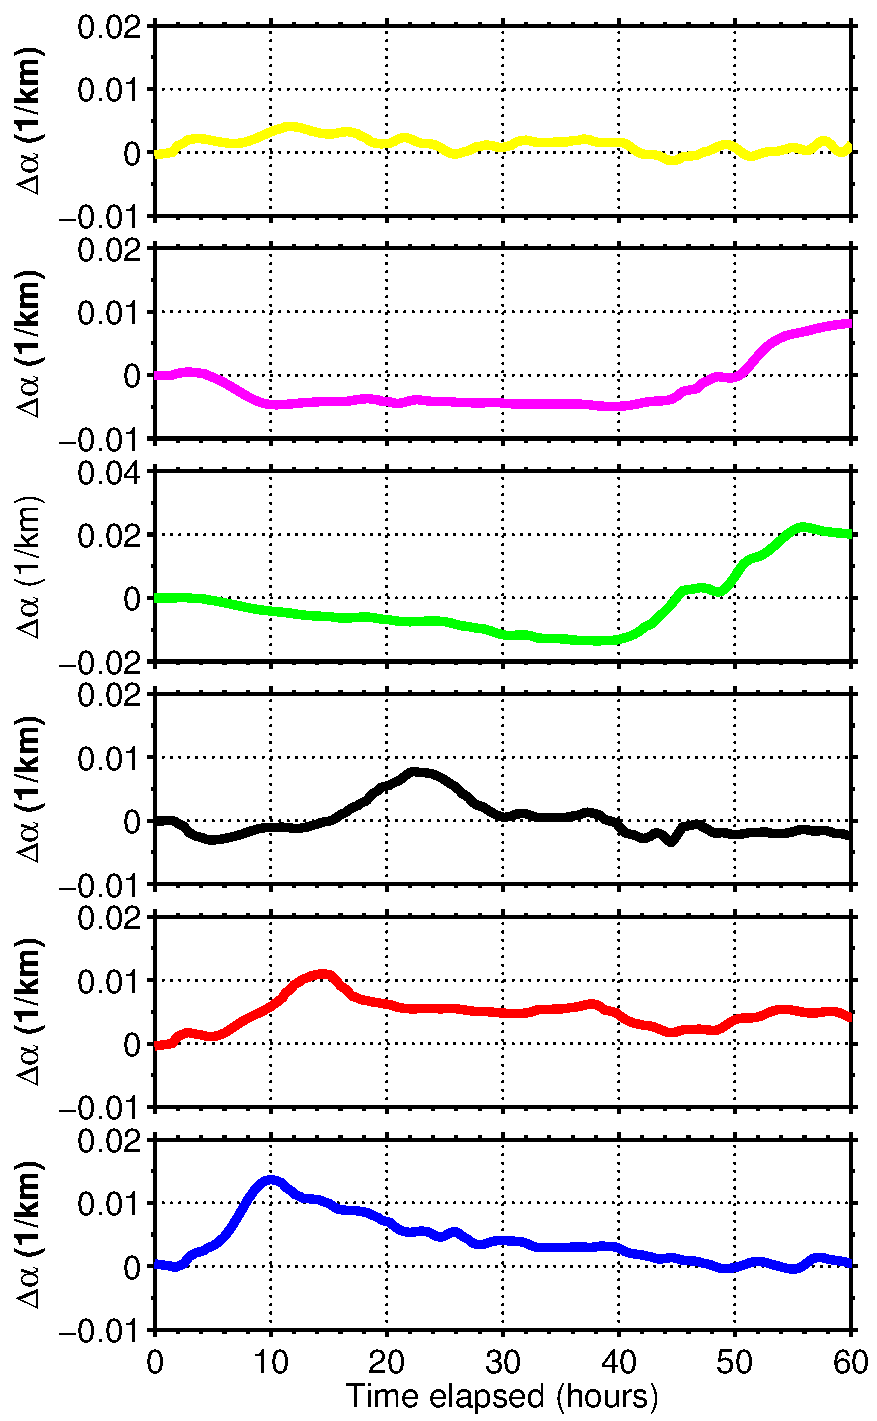
\includegraphics[width=0.4\textwidth]{Fig/fig4}
   \caption{Top: forward propagation in attenuating media; Bottom: backpropagation wavefield in attenuating media with attenuation compensation. The red star denotes an explosive source and the black triangulars denote receivers. The label \textbf{H} and \textbf{L} represent high frequencies and low frequencies signals. To correctly account for attenuation effects (including absorption and phase dispersion), the absorption term must be reversed so as to amplify the signal as time progresses. In contrast, the dispersion term (dependence of the sound speed on frequency) must remain unchanged.}
 \end{figure}
 
\section{Conclusions}
We have presented measurements of seismic attenuation changes from active crosswell seismic waveform at the 6 receivers in the Frio-II site. Calculations of seismic attenuation changes are based on theory of centroid frequency shift. With all 6 receivers, three features in attenuation changes during the first 60 hr of CO$_2$ injection: (1) attenuation peak at different times; (2) increase-decrease attenuation pattern across receivers; (3) no systematic attenuation change at the top receiver. Seismic attenuation change presents a potential opportunity to quantify the CO$_2$ saturation using seismic data. Further rock physics study will be valuable to link attenuation to saturation for estimates of CO$_2$ saturation in the spatial-temporal domain.

\section{Acknowledgments}
This work was supported by the GEOSEQ project for the Assistant Secretary for Fossil Energy, Office of Coal and Power Systems through the National Energy Technology Laboratory, of the U.S. Department of Energy, under contract No. DE-AC02-05CH11231. Zhu is financially supported by the Postdoctoral fellowship in the Jackson School of Geosciences at the University of Texas at Austin.
\onecolumn

\bibliographystyle{seg}
\bibliography{refs}
